\section*{Question 3}
\emph{Investigate the solutions when the viscosity is very small (in effect, zero) so that we reduce to the one-dimensional wave equation. Look the amplitude (growth/decay, stability) and dispersion (phase speed of wave components. One way to retain stability is to add an optimal small amount of artificial viscosity (e.g. the Lax-Wendroff method, Euler+CDiff2, using $\nu_{Euler} = 0.5 c^2 dt, \nu_{RK2} = 0.03 c^4 dt^3/dx^2$).}

When viscosity is $\approx 0$ (figure \ref{visco}) the solution tends to explode as the energy and area go to infinity due to numerical error. The reason for this is that some gain exists due to numerical approximation that is accumulated with each iteration. The effect is strongest in Euler based methods of time propagation since any previous errors will be added to the new time step. RK2 is much better behaved and the errors accumulate more slowly (from \ref{visco} it seems to be linear), thus requiring many more time steps to reach infinity values.

\begin{figure}[!htb]
\centering
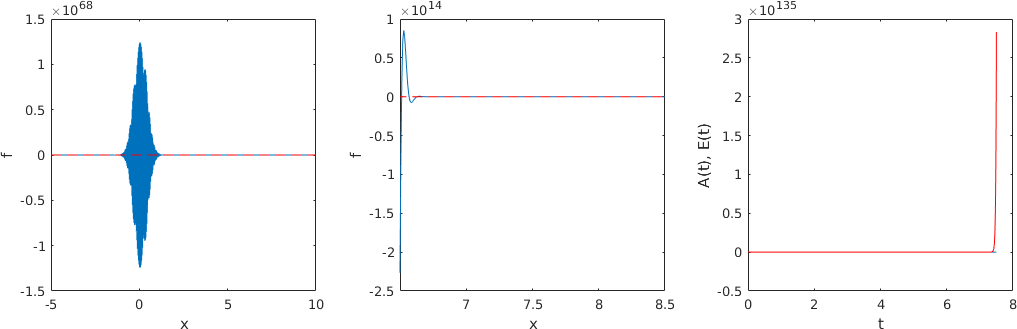
\includegraphics[scale=0.6]{./TEXT/visc01.png}
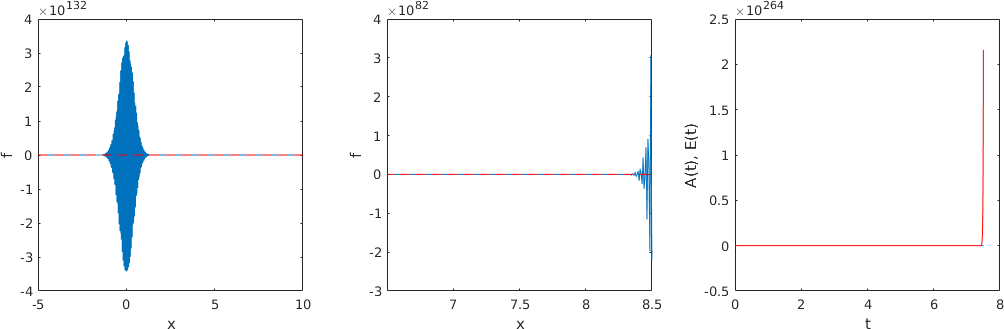
\includegraphics[scale=0.6]{./TEXT/visc02.png}
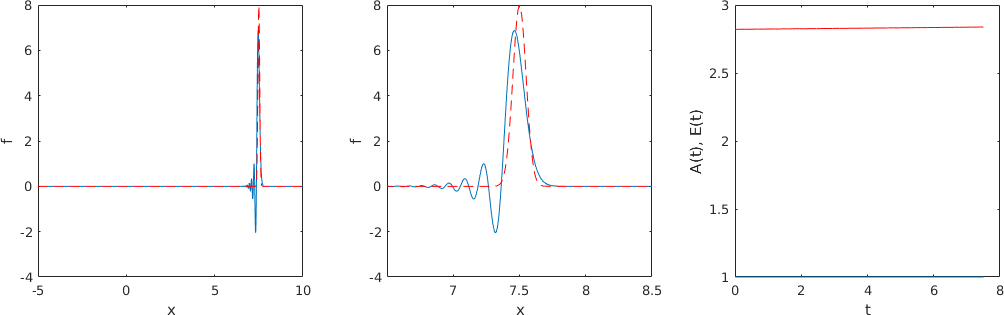
\includegraphics[scale=0.6]{./TEXT/visc03.png}
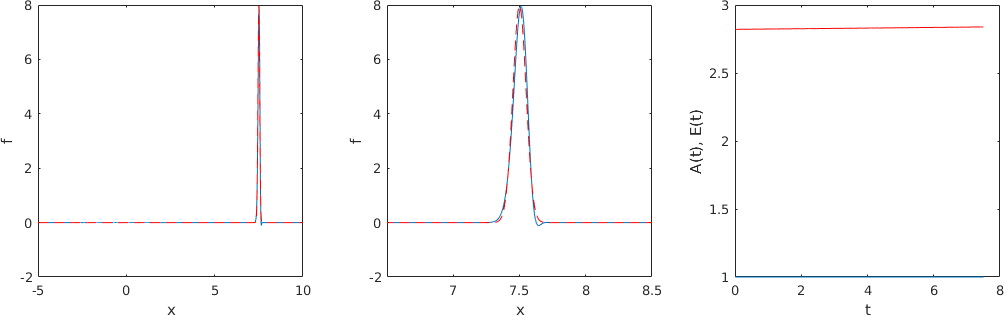
\includegraphics[scale=0.6]{./TEXT/visc04.png}
\caption{Behaviour of the numerical schemes for a viscosity $\nu = 0$: \nth{1} Euler-CD2, \nth{2} Euler - CD4, \nth{3} RK2 - CD2 and \nth{4} RK2 - CD4}
\label{visco}
\end{figure}

The Lax-Wendroff artificial viscosity stabilises all discretisation methods but it introduces inaccuracies in the simulation. Figure \ref{lax} shows that the four methods are stable (i.e. energy does not increase), but for all cases except Euler with \nth{4} order central differences some energy is dissipated, thus it is not in agreement with the physics requirement and the solution cannot be deemed accurate. A solution to this may be to adaptively change the $0.5$ or $0.03$ constants to avoid this behaviour and keep energy constant. 

\begin{figure}[Ht!]
\centering
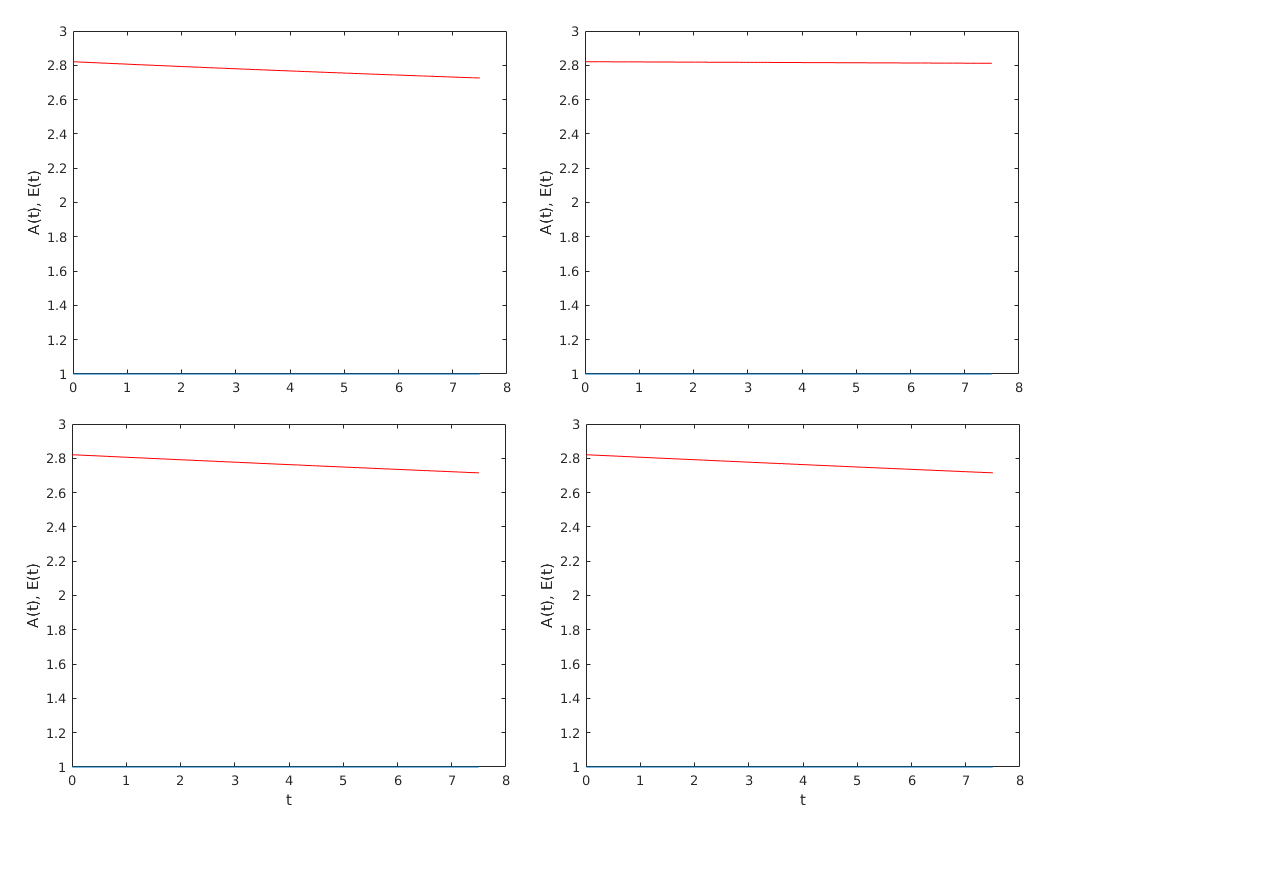
\includegraphics[scale=0.6]{./TEXT/lax.png}
\caption{Energy and Area variation when the Lax-Wendroff artificial viscosity is used.}
\label{lax}
\end{figure}